\documentclass{report}

\usepackage{fullpage}
\usepackage{url}
\usepackage{verbatim}
\usepackage{graphicx}
\usepackage{parskip}
\usepackage{pdfpages}
\usepackage[style=ieee,sorting=none,dateabbrev=false,backend=biber]{biblatex}
\addbibresource{report.bib}

\title{Smartwatch Gesture Recognition}
\date{\today}
\author{
  Lucas Wojciechowski \& Dane Carr \& Ariel Weingarten \\
  Group 15
}

\begin{document}

\maketitle

% The common requirement for all project is that the students in each group need to make use in their design project any method or combination of methods of material taught in the course (or closely related to it) to solve the proposed problem or improve on an existing solution. These are the required deliverables
% A report of 20 to 25 pages needs to be provided with these sections:

\chapter{Abstract}

% Abstract

\chapter{Problem Statement and Solution Motivation}
Wearable technology, such as smartwatches, are poised to become a ubiquitous consumer product. According to businessinsider.com, smartwatches sales are projected to reach 90 million units by 2018 \cite{BusinessInsider}. Many user interface paradigms still need to be rethought for these devices to accommodate their small screens and limited input methods. 

\begin{figure}[ht!]
  \label{smartwatch}
  \centering
  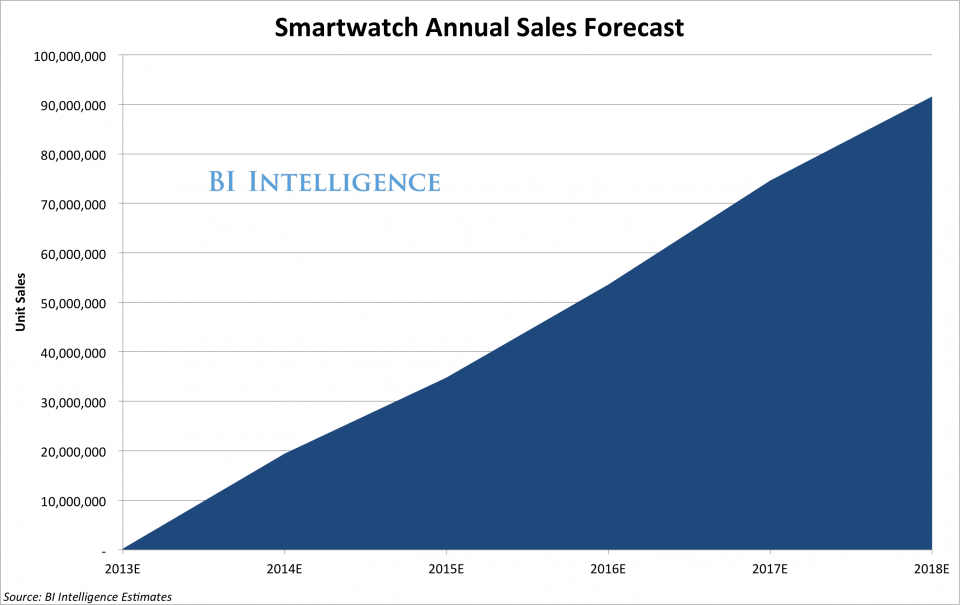
\includegraphics[width=90mm]{smartwatch.png}
  \caption{Smartwatch Annual Sales Projection \label{overflow}}
\end{figure}

Currently, these devices rely mostly on touch input and voice control. Touch input is usually effective, but due to the small form factor, a significant portion of the screen is often obscured by the user's finger. Voice control can be used to complete more complex actions that might be tedious to complete using only touch input, but voice commands are not always practical. They may be less effective in noisy environments, or users might feel uncomfortable using them in public places due to issues with privacy and social acceptance.

Hand and arm gestures could be used to augment existing input paradigms. Though less expressive than voice commands, hand and arm movements are relatively private and they are a natural way to communicate with the environment. There are presently no publicly available gesture recognition solutions for off-the-shelf smartwatches, though theories and interface ideas have been prototyped with other sensors such as Microsoft Kinect or custom ultra-sound detection systems. The potential applications of this technology are far-reaching, from seamless control of Internet-of-things devices to accessibility for visually impaired users.

We have acquired a LG G Watch R and a Nexus 5 phone to record gesture data via a simple, custom-built Android application. Data collected from the watch's accelerometer will be used to train a neural network to classify a set of simple gestures. We will compare the accuracy and performance of our classifier against similar gesture recognition systems in the research community.

\chapter{Theoretical Background Material}
Our work is inspired by two works in particular. First, there is the famous ``Learning Representations by Back-Propagating Errors" paper that first introduced the back propagation algorithm. Second, there is ``Gestures without Libraries, Toolkits, or Training: A \$1 Recognizer for User Interface Prototypes". The former lays the groundwork for our solution and the latter provided motivation for the problem domain.

\section{Backpropagation}

Backpropagation has become a common method for training neural networks. Before its formulation,  there was no way to provide a measure of accuracy for hidden layers in neural networks.

It is most often used in the supervised learning process as it requires the expected labeling for a set of inputs.  Before the formulation of this algorithm there

\section{\$1 Recognizer}s

% Theoretical background material with references

\begin{figure}[ht!]
  \label{gestures}
  \centering
  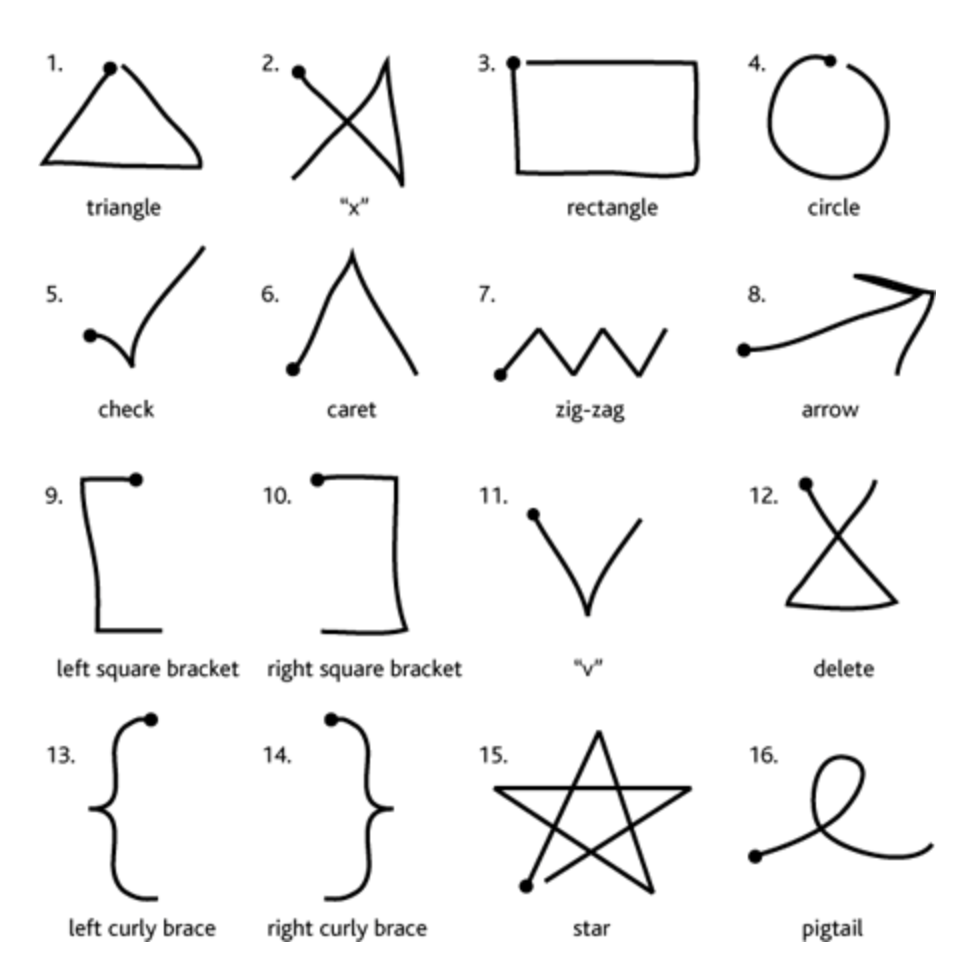
\includegraphics[width=90mm]{gestures}
  \caption{Gestures supported by the \$1 Recognizer}
\end{figure}

\chapter{Solution}

% Present your solution using tool(s) learned in class (or something related)

% TODO good transition from previous section
We set out to build a system which would allow us experiment with smartwatch gesture recognition.

As a research platform, this system was designed to be extensible, simple, and easy to work with. As a potential consumer platform, this system was built to be portable and permanent enough to run natively on Andorid smartphones.

Due to the lack of prior art in this space, we had to build some fundamental infrastructure ourselves, such as a data collection system and data repository for the smartwatch gesture sensor data.

In the end, the system we built consists of the following components
\begin{enumerate}
\item a set of gestures that were easy to perform by users and easy to recognize by our machine
\item a data collection app collected smartwatch sensor data from users performing our gestures
\item a repository of training and testing data sets from the collection app
\item a custom neural network implementation designed for performance and portability on Android smartphones
\item a testing harness which replayed the data to train and test a neural network for gesture recognition
\item a neural network topology optimizer based on genetic algorithms
\end{enumerate}

In the following subsections, we will discuss the requirements and implementation of each component in detail.

\section{Gesture Set}

% Which gestures worked and which gestures didn't work?

We decided to use a subset of the gestures defined in the ``\$1 Unistroke Recognizer" paper, as discussed above and pictured in \ref{gestures}. Using this set of gestures was a good solution to our problem because
\begin{itemize}
\item they have become the canonical gesture set in the industry, so using them would allow us to directly compare our results to other's
\item they are well suited, semantically, to act as user input for mobile applications
\item they are know to be easily recognizable by algorithms
\item they are easy to draw for users
\end{itemize}

In addition to these gestures, we considered including a number of ``flick" gestures, rapid arm movements from the neutral position, in which the user's arm is by their side, to a direction (forwards, outwards, backwards). It was thought that these gesture would also be useful as a semantic user input technique, allowing for direct manipulation of virtual interfaces or quick activation of functionality. After some experimentation, however, we found these gestures were not well suited to identification by our neural network. We theorize this may be due to the relatively short duration of these gestures. A ``flick forwards" gesture might only take 100 milliseconds to perform, while most of the \$1 Recognizer gestures take 1 to 2 seconds. This very short burst of accelerometer data may look like background noise to the neural network or just be too different a classification task. Further work could be done in this area.

In the end, we chose to focus on the recognition of the following gestures based on their user approachability and our neural network's ability to differentiate between them
\begin{itemize}
\item circle
\item triangle
\item check
\item pigtail
\item arrow
\item star
\end{itemize}

\section{Data Collection App}

We had to collect a data set in order to train and test our nerual network.


To this end, we built an Android app which would prompt users to draw a particular gesture, vibrate their watch to indicate the beginning of the data collection period, collect data from all smartwatch sensors during the data collection period, vibrate again to indicate the end of the collection period, and store the data for later analysis. This app was designed to be used either directly by the user wearing the smartwatch or in a ``researcher and research subject" setting.

% TODO ARIEL expand on the Android Apis we used here. What is Android wear?

\begin{figure}[ht!]
  \label{app}
  \centering
  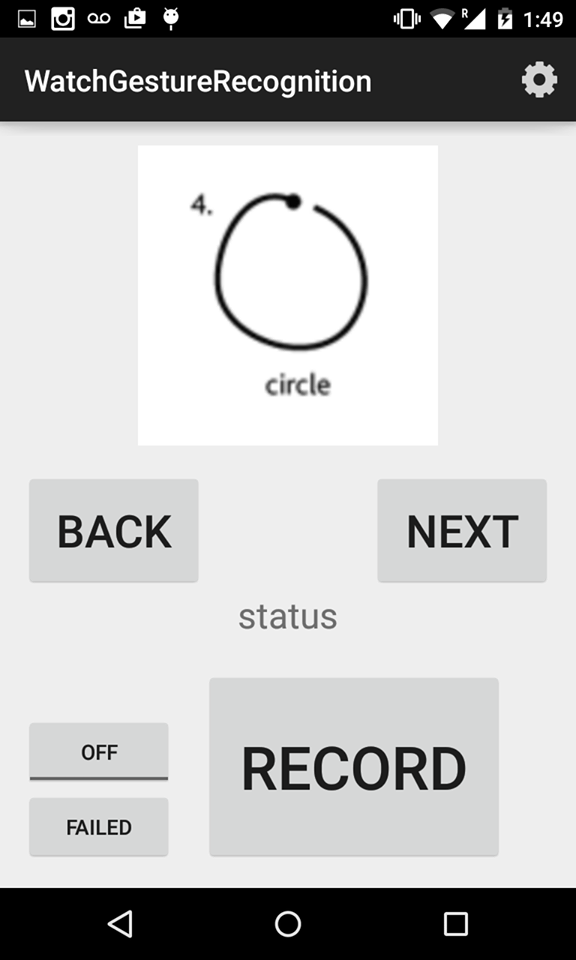
\includegraphics[width=90mm]{app}
  \caption{Screenshot of Android smartwatch sensor data collection app}
\end{figure}


The app interface is pictured in \ref{app}. % TODO ARIEL explain user interface

The smartwatch we used, the LG R Watch, reported data from the three different sensors
\begin{itemize}
\item accelerometer
\item gyroscope
\item magnetometer (compass)
\end{itemize}
In addition, it reported data from a virtual ``orientation" sensor, which was a composite of the other sensors in a more intuitive reference frame.

While we collected data from all these sensors, our neural network seemed to perform best on the accelerometer data alone.

\section{Repository of Testing and Training Data}

\section{Neural Network Implementation}

% How did we format the data for input to the NN?

\section{Testing Harness}

\section{Topology Optimizer}

% How did we determine the optimal toplogy?
% What was the optimal topology?
% What were the performance implications of larger / smaller toplogies

\chapter{Results}

\section{Codebase Metrics}

% How many lines of code do we have?

\section{Training Performance}

% CPU cost of training
% Number of data points needed to train system
% Difficulty of collecting data

\section{Classification Performance}

% Performance relative to the $1 Recognizer

\chapter{Conclusion}

% Conclusion

\chapter{References}

% References
\printbibliography

\end{document}
